\documentclass[9pt]{IEEEtran} % Using 9pt font size

% --- Standard Packages ---
\usepackage[english]{babel}
\usepackage{graphicx}
\usepackage{float}        % For [H] placement specifier
\usepackage{amsmath}
\usepackage{array}        % For table column definitions
\usepackage{hyperref}     % For clickable references/links
\usepackage{xcolor}       % For colored links (used by hyperref)
\usepackage[utf8]{inputenc} % Use utf8 encoding
\usepackage[T1]{fontenc}    % Font encoding
\usepackage{lmodern}      % Use Latin Modern fonts
\usepackage{siunitx}      % For aligned numbers in tables
\usepackage{booktabs}     % For nicer table rules (\toprule, \midrule, \bottomrule)
\usepackage{caption}      % For better control over captions
% \usepackage{subcaption}   % If you want subfigures later (not used for this version)

% --- Hyperref Setup ---
\hypersetup{
    colorlinks=true,
    linkcolor=blue,
    filecolor=magenta,
    urlcolor=cyan,
    pdftitle={Parallel 2D Gray-Scott Simulation using MPI},
    pdfauthor={Erik Pahor, Jaka Škerjanc} 
}

% --- Graphics Path ---
\graphicspath{{./figures/}} % Make sure you have a 'figures' subdirectory or adjust
\DeclareGraphicsExtensions{.pdf,.png,.jpg}

% --- Hyphenation ---
\hyphenation{op-tical net-works semi-conduc-tor Gray-Scott MPI OpenMPI}

% ============================================================================================
\title{\vspace{0ex}
Parallel 2D Gray-Scott Simulation using MPI}

\author{Erik Pahor, Jaka Škerjanc\vspace{-3.5ex}} 
% ============================================================================================

\begin{document}

\maketitle
\thispagestyle{empty} % Remove page number from first page

\section{Introduction}
\label{sec:introduction}

This report details a parallel implementation of the 2D Gray-Scott reaction-diffusion model using C++ and the Message Passing Interface (MPI). The Gray-Scott system is known for generating complex and visually interesting patterns arising from the interaction of two chemical species. The primary objective of this work was to accelerate the computationally intensive simulation by distributing the workload across multiple processor cores on a distributed memory system. A parallel MPI version was developed, employing finite differences for spatial discretization, the forward Euler method for time integration, and periodic boundary conditions. The parallelization strategy uses a row-wise domain decomposition. Performance was benchmarked on the Arnes HPC cluster across various grid sizes and core counts. The focus is on execution time and speedup ($S=t_s/t_p$), where $t_s$ is the execution time of an equivalent sequential C implementation and $t_p$ is the execution time of the parallel MPI version.

\section{Implementation Approach}
\label{sec:implementation}

\subsection{Gray-Scott Model and Discretization}
The simulation solves the Gray-Scott partial differential equations. The spatial domain is an $N \times N$ grid. The Laplacian operator ($\nabla^2$) is approximated using a standard 5-point finite difference stencil. Concentrations $U$ and $V$ are updated over discrete time steps $\Delta t$ using the forward Euler method with periodic boundary conditions.

\subsection{Parallel MPI Implementation}
The parallel version was implemented using C++ and the OpenMPI library. The core parallelization strategy is based on domain decomposition:

\textbf{Row-wise Decomposition:} The global $N \times N$ grid is divided into horizontal strips, with each MPI process assigned one such strip.

\textbf{Halo Exchange:} To compute the Laplacian at strip boundaries, processes exchange halo (ghost cell) rows with their upper and lower neighbors. Non-blocking $MPI\_Isend$ and $MPI\_Irecv$ followed by $MPI\_Waitall$ were used.

\textbf{Double Buffering:} Each MPI process uses two local buffers for each species (U and V) for time steps $n$ and $n+1$. Pointers are swapped after each time step.

\textbf{Data Aggregation for Output:} The final V grid is gathered onto rank 0 using $MPI\_Gatherv$ for saving as a PGM image.

\section{Experimental Setup}
\label{sec:setup}

Tests were conducted on the Arnes HPC cluster. The MPI C++ code was compiled using $mpicc$ (GCC) with $-O3$. Fixed parameters: $\Delta t = 1.0$, $D_u = 0.16$, $D_v = 0.08$. The (F, k) parameters were (0.060, 0.062) ("Default" pattern). Benchmarks ran for 5000 steps on grids $256^2$ to $4096^2$, using 1, 2, 4, 16, 32, and 64 cores. MPI execution times ($t_p$) were measured on rank 0 using $MPI\_Wtime$, including computation and final data gathering. Sequential times ($t_s$) were obtained from a separate, non-MPI C implementation run on a single core. 

\section{Results and Discussion}
\label{sec:results_discussion}

Execution times ($t_p$) for the MPI implementation are in Table~\ref{tab:mpi_times}. Speedup ($S = t_s/t_p$) relative to the sequential C implementation is in Table~\ref{tab:mpi_speedups}. Figure~\ref{fig:speedup_plot_mpi} graphically presents these speedups. An example visualization is in Figure~\ref{fig:vis_example_mpi}.

% --- MPI Execution Times Table (tp) ---
\begin{table}[H]
\centering
\caption{MPI Execution Times ($t_p$ in seconds) for 5000 steps.}
\label{tab:mpi_times}
\sisetup{round-mode=places,round-precision=3} 
\resizebox{\columnwidth}{!}{%
\begin{tabular}{c S[table-format=3.3] S[table-format=3.3] S[table-format=3.3] S[table-format=3.3] S[table-format=3.3] S[table-format=3.3]}
\toprule
Grid Size & \multicolumn{6}{c}{Number of Cores ($p$)} \\
\cmidrule(lr){2-7}
          & {1}      & {2}      & {4}      & {16}     & {32}     & {64} \\
\midrule
$256^2$   & 3.60096  & 2.22889  & 1.35506  & 0.534491 & 0.366059 & 145.375 \\
$512^2$   & 11.8407  & 6.48054  & 3.86730  & 1.57683  & 1.01023  & 0.912569 \\
$1024^2$  & 62.4339  & 32.0298  & 18.8706  & 6.99392  & 4.35307  & 2.71798 \\
$2048^2$  & 239.252  & 121.123  & 62.8751  & 20.1589  & 11.6466  & 11.5991 \\
$4096^2$  & 801.418  & 401.763  & 219.462  & 109.845  & 84.6429  & 115.078 \\
\bottomrule
\end{tabular}%
}
\end{table}

% --- Sequential Times (ts) ---
% ts_256 = 3.65
% ts_512 = 12.38
% ts_1024 = 65.05
% ts_2048 = 258.33
% ts_4096 = 867.52

% --- MPI Speedups Table (S = ts/tp) ---
\begin{table}[H]
\centering
\caption{MPI Speedup ($S = t_s/t_p$) vs. Sequential C.}
\label{tab:mpi_speedups}
\sisetup{round-mode=places,round-precision=2} 
\resizebox{\columnwidth}{!}{%
\begin{tabular}{c S[table-format=1.2] S[table-format=2.2] S[table-format=2.2] S[table-format=2.2] S[table-format=2.2] S[table-format=3.2]}
\toprule
Grid Size ($t_s$) & \multicolumn{6}{c}{Number of Cores ($p$)} \\
\cmidrule(lr){2-7}
                 & {1}    & {2}    & {4}    & {16}   & {32}   & {64} \\
\midrule
$256^2$ (3.65s)  & 1.01   & 1.64   & 2.69   & 6.83   & 9.97   & 0.03 \\ % 3.65/tp
$512^2$ (12.38s) & 1.05   & 1.91   & 3.20   & 7.85   & 12.25  & 13.57 \\ % 12.38/tp
$1024^2$ (65.05s)& 1.04   & 2.03   & 3.45   & 9.30   & 14.94  & 23.93 \\ % 65.05/tp
$2048^2$ (258.33s)& 1.08  & 2.13   & 4.11   & 12.82  & 22.18  & 22.27 \\ % 258.33/tp
$4096^2$ (867.52s)& 1.08  & 2.16   & 3.95   & 7.90   & 10.25  & 7.54 \\ % 867.52/tp
\bottomrule
\end{tabular}%
}
\end{table}

\begin{figure}[H]
    \centering
    % YOU NEED TO CREATE THIS PLOT BASED ON THE MPI DATA IN TABLE 2 (new speedups)
    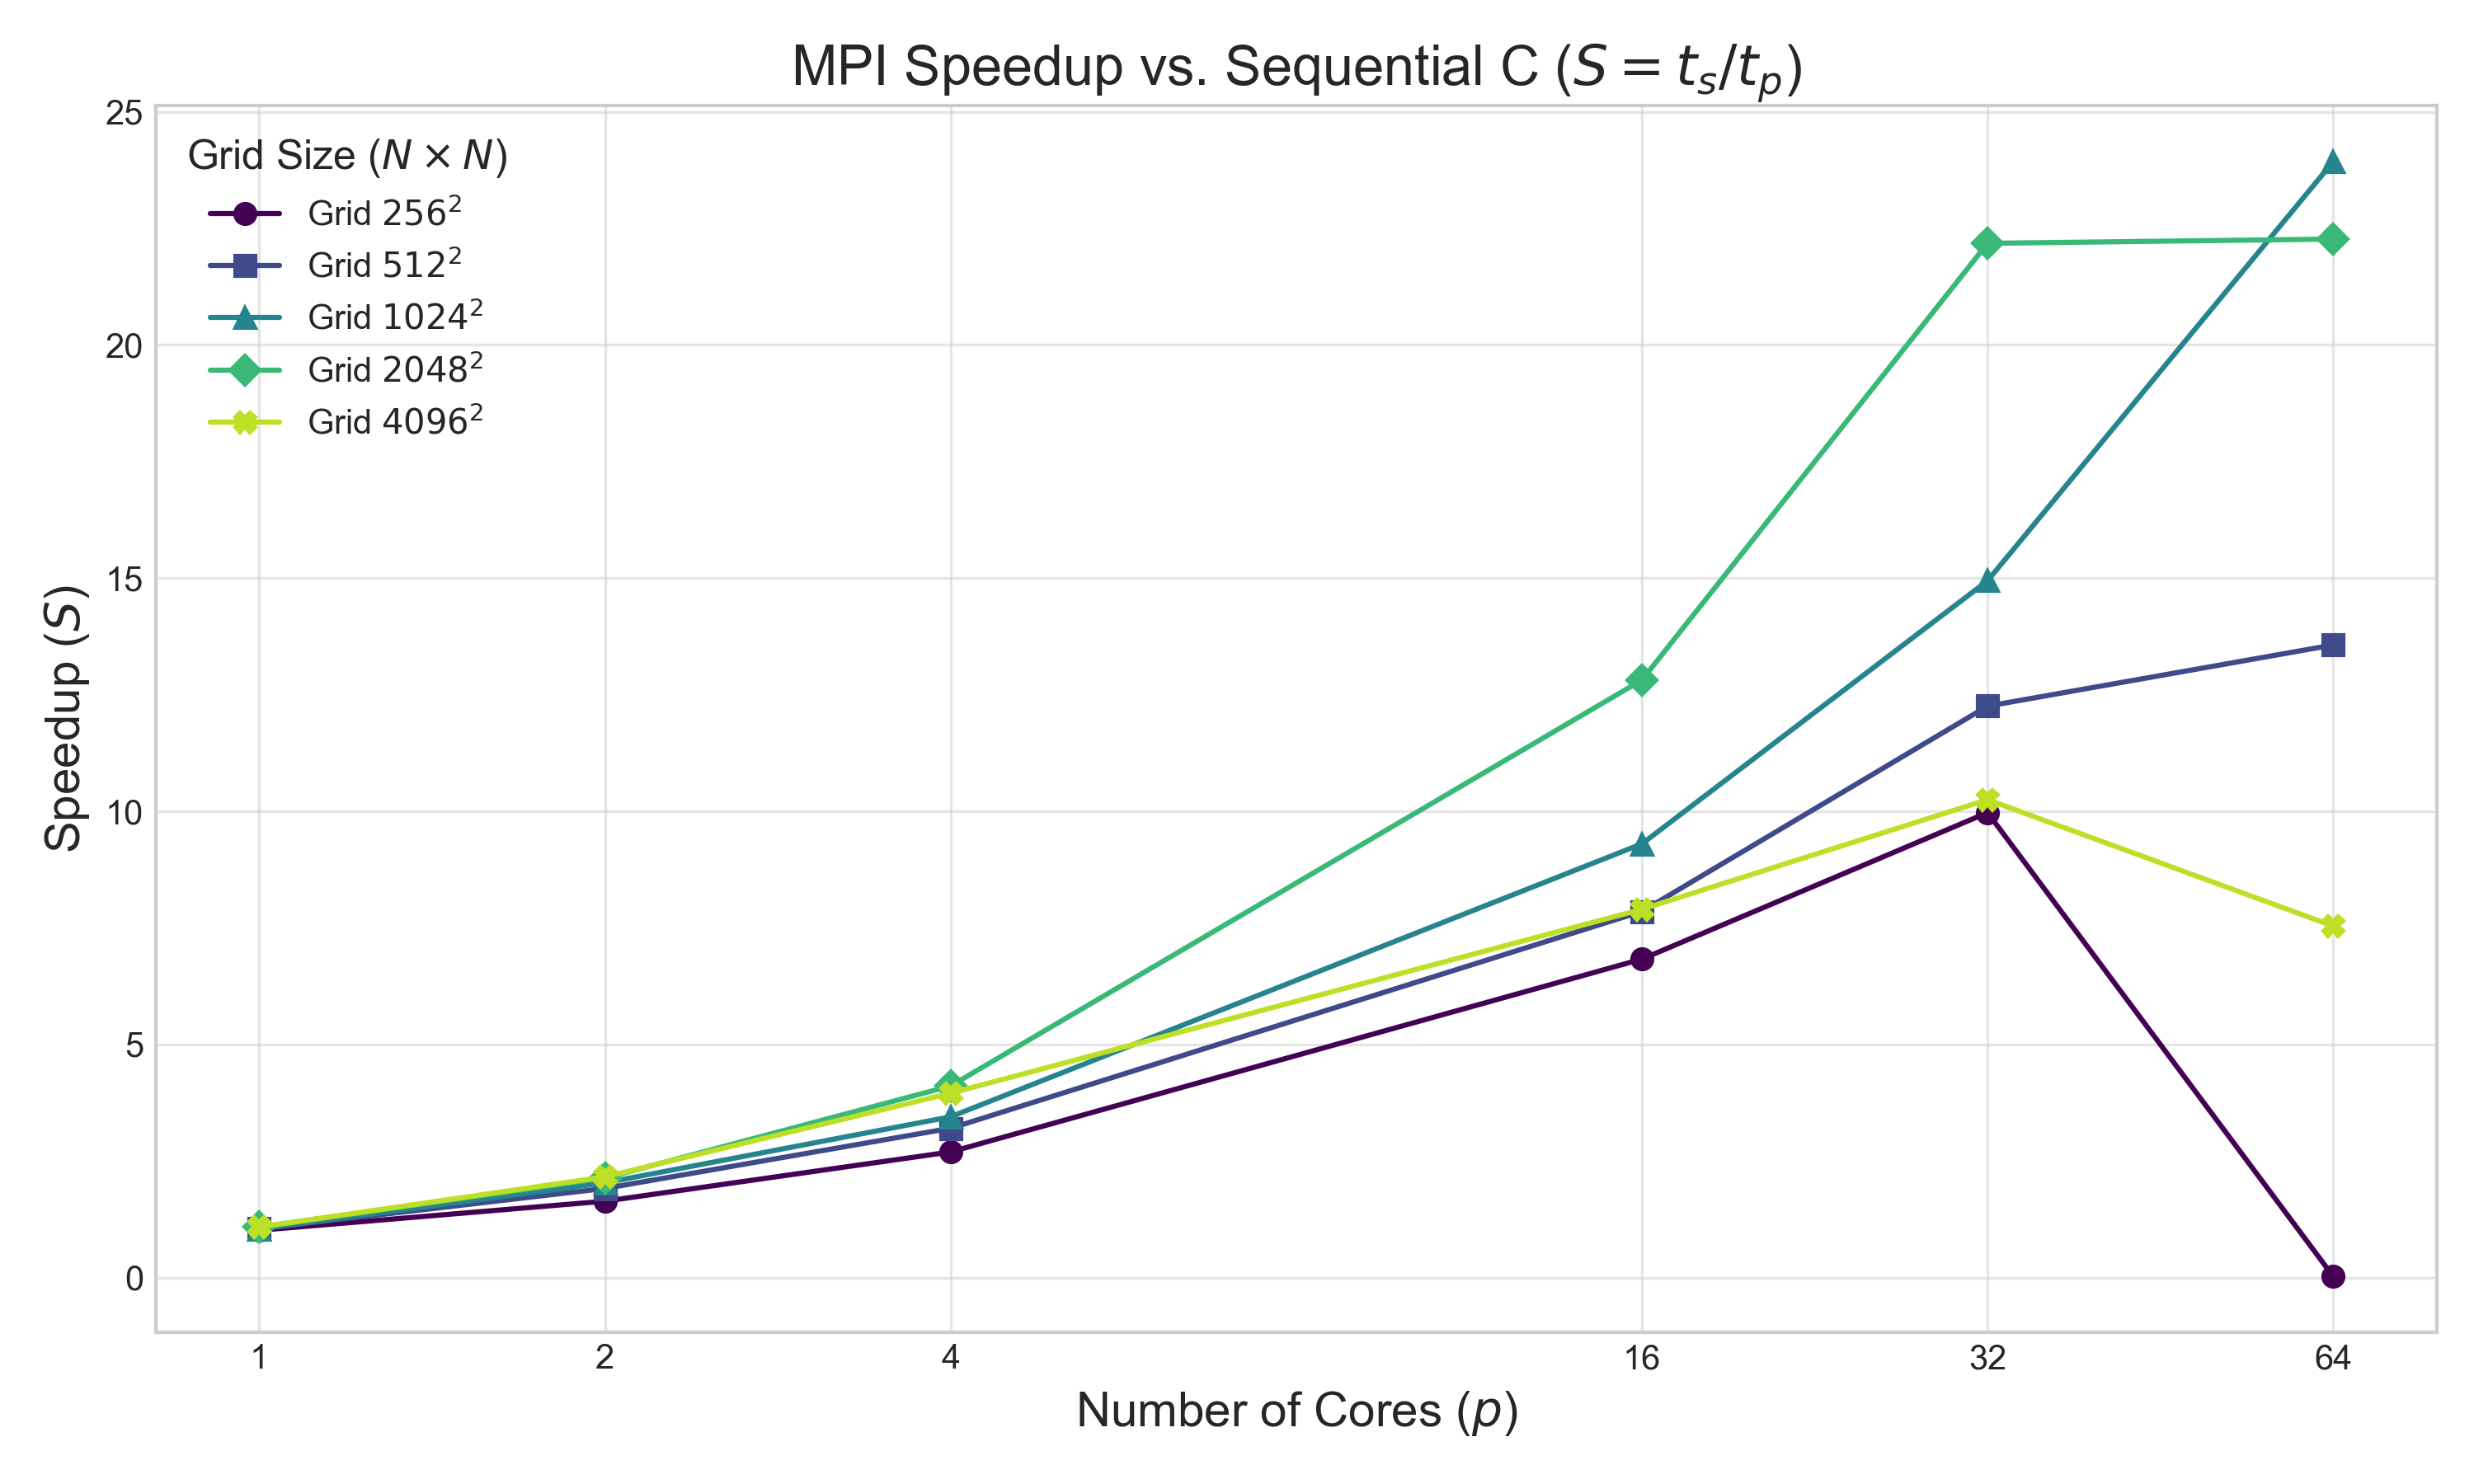
\includegraphics[width=0.9\columnwidth]{mpi_speedup_plot_vs_seq1.png} 
    \caption{Speedup of MPI implementation relative to sequential C execution ($S=t_s/t_p$).}
    \label{fig:speedup_plot_mpi}
\end{figure}

\begin{figure}[H]
    \centering
    
\includegraphics[width=0.7\columnwidth]{default.png} 
    \caption{Species V concentration for 'Default' pattern (F=0.060, k=0.062), $N=256$, 5000 steps, visualized from MPI simulation.}
    \label{fig:vis_example_mpi}
\end{figure}

The MPI implementation achieves notable speedups over the sequential C code, especially for larger grid sizes and an optimal number of cores. For example, the $1024^2$ grid shows a speedup of approximately $23.9\times$ with 64 cores. The $2048^2$ grid achieves a speedup of $22.2\times$ with 32 cores. Even the MPI version running on a single core ($p=1$) is slightly faster than the pure sequential C code in some cases ($t_s/t_{p,1} > 1$), which might be attributed to differences in compiler optimizations or minor structural differences, though ideally, $t_{p,1}$ should be very close to $t_s$ plus minimal MPI overhead.

However, the limitations of strong scaling are evident. For the $256^2$ grid, performance degrades drastically at 64 cores, yielding a speedup far less than 1. This indicates that the problem size per core is too small, and communication overheads (halo exchanges) overwhelm any benefits from parallel computation. A similar, albeit less severe, trend is seen for $4096^2$ at 64 cores, where speedups are lower than with 32 cores. This saturation or decline in speedup at higher core counts for a fixed problem size is expected due to Amdahl's Law, as the inherently sequential portions of the algorithm and the communication costs become dominant.

The row-wise decomposition distributes the computational load. Non-blocking communication ($MPI\_Isend$/$MPI\_Irecv$ with $MPI\_Waitall$) is used to avoid deadlocks. The overall results suggest that the MPI parallelization is beneficial, but careful consideration of the problem size relative to the number of cores is necessary to achieve efficient parallel execution.

\section{Conclusion}
\label{sec:conclusion}

The MPI-based parallel solver for the 2D Gray-Scott model demonstrates significant acceleration compared to a sequential C implementation. Using row-wise domain decomposition and halo exchanges, speedups of up to $\approx 24\times$ (for $1024^2$ on 64 cores) were achieved. The effectiveness of the parallelization is highly dependent on the grid size and the number of cores, with larger problems generally exhibiting better scalability.

The study highlights the critical role of the computation-to-communication ratio. For configurations where this ratio is low (small grids on many cores), communication overheads significantly impede performance, sometimes resulting in slowdowns compared to fewer cores or even the sequential version. This underscores a fundamental challenge in distributed memory parallel computing. The developed MPI solution provides a viable method for accelerating large-scale Gray-Scott simulations.

\end{document}